\uuid{Cmh5}
\exo7id{5099}
\auteur{rouget}
\organisation{exo7}
\datecreate{2010-06-30}
\isIndication{false}
\isCorrection{true}
\chapitre{Continuité, limite et étude de fonctions réelles}
\sousChapitre{Etude de fonctions}

\contenu{
\texte{

}
\begin{enumerate}
    \item \question{Etudier brièvement la fontion $x\mapsto\frac{\ln x}{x}$ et tracer son graphe.}
\reponse{Pour $x>0$, posons $f(x)=\frac{\ln x}{x}$. $f$ est définie et dérivable sur $]0,+\infty[$ et, pour $x>0$,
$f'(x)=\frac{1-\ln x}{x^2}$. $f$ est donc strictement croissante sur $]0,e]$ et strictement décroissante sur
$[e,+\infty[$. Le graphe de $f$ s'en déduit facilement~:

$$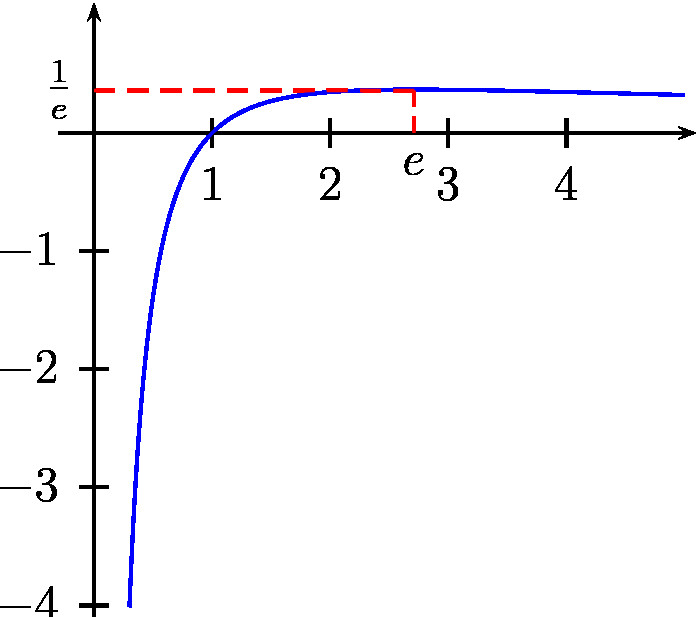
\includegraphics{../images/img005099-1}$$}
    \item \question{Trouver tous les couples $(a,b)$ d'entiers naturels non nuls et distincts vérifiant $a^b=b^a$.}
\reponse{Soient $a$ et $b$ deux entiers naturels non nuls tels que $a<b$. On a alors

$$a^b=b^a\Leftrightarrow\ln(a^b)=\ln(b^a)\Leftrightarrow b\ln a=a\ln b\Leftrightarrow\frac{\ln a}{a}=\frac{\ln b}{b}\Leftrightarrow f(a)=f(b).$$
Si $a\geq3$, puisque $f$ est strictement décroissante sur $[e,+\infty[$, on a alors $f(a)>f(b)$ et en particulier,
$f(a)\neq f(b)$. $a$ n'est donc pas solution.
$a=1$ n'est évidemment pas solution. Par exemple, $a^b=b^a\Rightarrow1^b=b^1\Rightarrow b=1=a$ ce qui est exclu.
Donc, nécessairement $a=2$ et $b$ est un entier supérieur ou égal à $3$, et donc à $e$, vérifiant $f(b)=f(2)$. Comme $f$
est strictement décroissante sur $[e,+\infty[$, l'équation $f(b)=f(2)$ a au plus une solution dans $[e,+\infty[$. Enfin,
comme $2^4=16=4^2$, on a montré que~:~il existe un et un seul couple $(a,b)$ d'entiers naturels non nuls tel que $a<b$
et $a^b=b^a$, à savoir $(2,4)$.}
\end{enumerate}
}
